
% Author: Andrew Gainer-Dewar, 2013
% This work is licensed under the Creative Commons Attribution 4.0 International License.
% To view a copy of this license, visit http://creativecommons.org/licenses/by/4.0/ or send a letter to Creative Commons, 444 Castro Street, Suite 900, Mountain View, California, 94041, USA.
\documentclass[twoside]{article}
\usepackage{ccpaper}
\usepackage{mathtools}
%\usepackage{graphcix}
% The Latin Modern font is a modernized replacement for the classic
% Computer Modern. Feel free to replace this with a different font package.
\usepackage{lmodern}

% Load in biblatex
% To use a different bibliography style, just change "numeric" to
% your preferred style (mla for MLA style, alphabetic for Author-Year
% style, etc.) There are a lot of options; check the BibLaTeX documentation.
\usepackage[backend=bibtex,style=numeric]{biblatex}
% Select the bibliography file
\addbibresource{sources.bib}

\title{The Hyperparameters of the Neural Nets}
%\subtitle{Subtitle of the paper} %Optional. Omit if not wanted.
\author{}
\date{}
\prof{}
\course{ Spring 2017}

% To enable double spacing, uncomment this line:
%\doublespacing

\begin{document}
\maketitle{}
%\title{The Hyperparameters of the Neural Nets}
The Artificial Neural Network is a powerful data-driven, self-adaptive, flexible computational tool possessing the capability of capturing nonlinear and complex underlying characteristics of any physical process with a high degree.\cite{wang2003artificial} It is due to this very nature that it is often seen as a "Black Box". These networks may seem to work autonomously for the most part, yet require human intervention at some level. Before the model learns the actual parameters, some "higher level" properties need to be set which define the complexity or the learning rate. It is these "knobs" of the big machine which are referred to as "Hyper-parameters". 

In \cite{bengio2000gradient}, the author defines the \textit{hyper-parameter} for a learning algorithm A as a variable to be set prior to the application of A to the data, one that is not directly selected by the learning algorithm itself. Choosing hyperparameter values is equivalent to the process of model selection. Hyperparameters may be discrete(as in model selection) or continuous. The values can be fixed by hand, or tuned by an algorithm,but it is essential that they are selected judiciously. Hyperparameter Optimization is a science as well as an art and this paper delves into the various mechanisms involved in the process.

Before digging deeper into hyperparameters, it is important to briefly consider the problems of overfitting and underfitting which are encountered while learning on neural networks.


Overfitting is a state when a machine learning algorithm captures the noise of the data. This happens when it learns on the training data too well , but fails to generalize it across other datasets.Hence it is a case of high variance and low bias.\cite{caruana2001overfitting} Quite often, overfitting is the result of an excessively complicated model.

Conversely, Underfitting which intuitively is the opposite of Overfitting , is a state where the learning algorithm misses the underlying pattern in the data. It can hardly perform well on the training set, let alone validation and tests. This is a good case where the learning model exhibits low variance but high bias. In practice, Overfitting is more of a problem, since it can show false hopes, and hyperparameter optimization is more relevant in fixing overfitting.

A commonly used method to avoid \textit{overfitting} is by using Regularization. Regularization adds a complex penalty to the loss function.\cite{girosi1995regularization}. It also helps in dealing with exploding gradients. Moreover, using Dropout has also been proved to be an effective method of preventing overfitting. The idea is to randomly remove some units during training. In \cite{srivastava2014dropout}, the authors discuss the advantages of dropout when compared to other regularization methods.
Throughout this literature, these terms will be frequently used, and it will be discussed how hyperparameter tuning helps in preventing overfitting and reducing overall error.


\section{Neural Network Hyperparameters}

Neural Networks can have a large number of  hyperparameters, some of which specify the structure of the network itself and some determine how the network is trained. Different neural networks may involve some different hyperparameters. The ones used in Feed-Forward Networks give a very good idea of the most important ones and there is plenty of literature on it, hence this essay focuses mainly on them. Mini Batch gradient descent is the optimizer of choice, due to it's popularity.



%\begin{enumerate}
\subsection{ Training method Hyperparameters:}
While Batch optimizers and Stochastic gradient descent optimizers have been two very popular gradient descent variants, the best of the two worlds is combined by the Mini batch gradient. The mini batch optimizer performs an update for every mini batch of n training examples:\newline
$\theta^{(t)} \leftarrow \theta^{(t - 1)} - \epsilon_t \frac{1}{B} \sum_{t^\prime = Bt + 1}^{B(t + 1)} \frac{\partial L(z_{t^\prime}, \theta)}{\partial\theta}$, 

where $z_{t^\prime}$  is example $t^\prime$ in the training set and the hyperparameters are the loss function L, the learning rate at step t$\epsilon_t$ , the mini-batch size $B$, and the number of iterations $T$ . $\theta^{(0)}$ is also a hyperparameter.

This way, it reduces the variance of the parameter updates, which can lead to more stable convergence; and  can make use of highly optimized matrix optimizations common to state-of-the-art deep learning libraries that make computing the gradient w.r.t. a mini-batch very efficient. Common mini-batch sizes range between 50 and 256, but can vary for different applications. Mini-batch gradient descent is quite often the algorithm of choice when training a neural network and the term Stochastic gradient descent is also is employed also when mini-batches are used.
\begin{itemize}

\item \textit{\textbf{Initial Learning rate}}

The learning rate is perhaps one of the most quintessential parameters to be tweaked. It determines how fast the gradient updates follow the gradient direction. When the rate is very small, the model converges slowly, and when the learning rate is too large, the model diverges. For neural networks with with standardized inputs bounded on [0,1], the learning rate is typically set between 1 and $10^-6$, and a good value to try is 0.01 \cite{bengio2012practical}.

The learning rate is typically reduced over time, the heuristic being that at first a descent parameter setting should be found, after which it must be fine tuned.
\item \textbf{\textit{Loss Function}}

The loss function compares the output of the network for a training example against the intended ground truth output. A typical loss function is the squared Euclidean distance, given by :
$L = \frac{1}{2} \sum_i (y_i - z_i)^2$

where $y_i$ is the output of the $i^{th}$ network output unit, and the $z_i$ is the $i^{th}$ value of the target output. The 1/2 is included by convention to make the gradient more simple. When the output is converted to a probability distribution, such as softmax, it is better to use the cross-entropy loss, given by: $L = -\sum_i y_i \log(z_i)$
\item \textit{\textbf{Mini batch size}} 

Choice of the mini-batch size $B$ is mostly computational: when it is larger, the updates can be computed more efficiently due to the use of parallel architectures; when $B$ is smaller, more updates can be made. In theory, this hyperparameter impacts the training time and not so much the test performance, so it may be optimized separately of the other hyperparameters. \cite{bengio2012practical} , e.g. it can first be set and fixed to a certain value a,d then the other hyperparameters, other than momentum, are optimized.

 
\item \textit{\textbf{Number of Training iterations}}

Perhaps the most common approach to setting this hyperparameter $T$ is by using the principle of early stopping. Early stopping simply stops training once the performance on a held-out validation set stops increasing. This can be a powerful way of preventing overfitting, to the point that it may make the choice of other hyperparameters trivial. \cite{bengio2012practical}. It also means that it hides the overfitting effect of other hyperparameters, possibly obscuring the analysis one may need to do whilst figuring out the effect of individual hyperparameters. For this reason, it is useful to turn early stopping off when analyzing effect of individual hyperparameters. \cite{bengio2012practical}
\item \textit{\textbf{Momentum}}

A common technique involved is to "smooth" out the gradient updates using a leaky integrator filter with parameter $\beta$ by 

$\bar{g} \leftarrow (1 - \beta)\bar{g} + \beta \frac{\partial L(z_t, \theta)}{\partial \theta}$

$\bar{g}$ can be used in place of the true gradient update in gradient descent. Some of the mathematically motivated approaches can ensure much faster convergence when using appropriate momentum, however for true stochastic gradient descent updates, ($\beta = 1$), with a harmonically decreasing learning rate is optimal \cite{bengio2012practical}


\item \textit{\textbf{Layer-specific optimization hyper-parameters}}

This method is not very common, yet sometimes appropriate and beneficial in context of layer wise unsupervised pre-training.\cite{bengio2012practical}. When the number of units per layer varies across the network, this method can provide useful. The idea is to set different values(such as learning rate) for different layers. 

\end{itemize}
\subsection{ Model Hyperparameters}
The structure of the neural network involves several hyperparameters in its design, which include the size and nonlinearity of each layer. The numeric properties of the weights are restricted in a way, and their initialization can have a strong effect on accuracy of the model. In addition the preprocessing of the input data is also important for ensuring convergence. Many hyperparameters can vary across layers, some of which are discussed below.
\begin{itemize}
\item \textit{\textbf{Number of Hidden Units}}
Each layer in the multi-layer feed forward network has a size that can be manually set and controlled.
Large hidden layers can allow the network to fit the training data well, and because regularization is typically used, it's mostly important to just use large hidden layers. Using the same size for all hidden layers generally works better or about the same as using a decreasing or increasing size. \cite{larochelle2009exploring}. The only downside to using higher number of hidden units is the added computation costs, and higher than optimal values hardly hurt the generalization performance. Additionally, using a first hidden layer which is larger than the input layer tends to work better. When using unsupervised pre-training, the layers should be made much bigger than when doing purely supervised optimization \cite{bengio2012practical}
\item \textit{\textbf{Weight Decay}}

In order to reduce overfitting, a regularization on the network weights is sometimes added to the training criterion(loss function). When encouraging the network weights $\theta$ to be close to zero, L2 regularization adds $\lambda_2 \sum_i \theta_i^2$ while L1 adds $\lambda_1 \sum_i |\theta_i|$ where $\lambda_2$ and $\lambda_1$ are the Lagrange multipliers that determine how important this regularization should be considered to be.\cite{bengio2000gradient}

This regularization could be viewed as a negative log-prior on the parameters. In the mini-batch case, the gradient of the regularization penalty should be multiplied by $B/T$, where $T$ is the training set size. In an online setting, $B/t$ should be used. L2 regularization corresponds to a Gaussian prior with variance $\sigma^2 = 1/(2\lambda_2)$, penalizing large weight values. L1 regularization corresponds to a Laplace density prior with a scale parameter $s = 1/\lambda_1$, acting as a form of feature selection \cite{bengio2012practical}.Wen both $L1$ and $L2$ are used, a different coefficient should be considered for each. A good reason to treat output weights differently to input weights is that it is known only output weight regularization suffices to constrain capacity. Another reason for treating them differently is due to the fact that they might be sparse. For instance, some input features might be 0 most of the time while others are non-zero, and the output weights from rarely active inputs should be more regularized than the ones from frequently observed units. \cite{bengio2012practical}  
\item \textit{\textbf{Activation Sparsity}}

Quite often the networks benefit from sparsity in hidden unit activations. A common way to enforce this is to use a L1 penalty( as discussed above) on the hidden unit parameters, provided that the activation has a saturating output around 0(such as sigmoid, and not tanh). Other common sparsity inducing regularizers include the Student-t $\log(1 + h_j^2)$, mean squared $\sum_j (\rho - \bar{h}_j)^2$ and KL-divergence $-\rho \log(\bar{h}_j) - (1 - \rho)\log(1 - \bar{h}_j) + C$ where $h_j$ is the $j^{th}$ activation of hidden layer $h$, $\bar{h}$ is the average activation over, e.g., a mini-batch, and $\rho$ and $C$ are additional hyperparameters. \cite{bengio2012practical}

\item \textit{\textbf{Non-Linearity}}

Some commonly used non-linearities include the sigmoid $1/(1 + e^{-a})$ which squashes the output into the range [0,1], $tanh \frac{e^a - e^{-a}}{e^a + e^{-a}}$ which is equivalent to sigmoid with range [-1, 1], the rectified linear unit (ReLU)max(0,a), and the step function. Sigmoid activation on the output later can cause issues with deep networks trained in a supervised fashion. Similarly "hard" units (ReLU and step) do not make sense for the output later, because when the output is saturated, no error gradient is passed back into the network. \cite{bengio2012practical}

\item \textit{\textbf{Weight Initialization}}

While weights are typically initialized to 0, the initialization can have a big impact on the local minimum found by the training algorithm. When chosen randomly, weights are often initialized in the range of $[-r,r]$ where $r$ is the inverse of the square root of the fain-in of the unit. For Restricted Boltzmann Machines, a zero mean Gaussian with a small standard deviation (0.1 or 0.01) should be used. Unsupervised pre-training can be seen as essentially a sophisticated initialization technique, which in most cases helps. Some of the common unsupervised initialization techniques used include greedily stacked RBMs(DBM) or de-noising/contractive auto-encoders.
\item \textit{\textbf{Seeds and model averaging}}

Many processes involved in training a neural network involve using a random number generator (e.g. random sampling of training data, weight initialization, etc). As a result of this, the seed passed to the random number generator can have an effect on the results. However, a different random seed can produce a non-trivially different model (even if it performs about as well). As a result, it’s common to train multiple models with multiple random seeds and then use model averaging (bagging, Bayesian methods) to improve performance.


\item \textit{\textbf{Preprocessing Input data}}

How the input data is prepared can have a profound impact on the learning and performance of the network. Element-wise standardization(subtracting the mean and dividing by standard deviation), Principal Component Analysis, uniformization(transforming each feature value to its approximate normalized rank or quantile), and nonlinearities such as log or square root are common preprocessing techniques.\cite{bengio2012practical}
\end{itemize}

This list of hyperparameters discussed is by no means exhaustive. These deal with Feed Forward Neural Networks mostly, yet also are generic to all. With varying architectures and learning methods, more choices arise. For instance, the denoising auto-encoder has a hyper-parameter scaling the amount of input corruption and the contractive auto-encoder has as hyperparameter a coefficient scaling the norm of the Jacobian of the encoder, i.e., controlling the importance of the contraction penalty. \cite{bengio2012practical}
%\end{enumerate}

\section{Hyperparameter Space Exploration}

The number of hyperparameters discussed above indicates that there are several choices that need to be made when creating a NN learning model. To achieve reproducibility, a principled approach needs to be used for setting the hyperparameters, or at least they must be explicitly stated in the model description. If a human is involved in the hyperparameter search, and the results are not explicitly stated, then they may not be reproducible.

Hyperparameter selection can be seen as both an optimization problem and a generalization problem(due to risk of Overfitting). It is especially difficult due to the computational cost \cite{bengio2012practical}; each hyperparameter setting being used to train a new model, and training being typically expensive. It has however been discovered that for some hyperparameters, the best setting may be obtained from a cheaper estimator(e.g, by randomly setting weights).

In most cases, a range of values is tried for each hyperparameter. It’s always possible that the best value falls on the edge of this range, which may indicate that a better value lies outside of the range. Due to non- convexity, however, a “best” value on the interior of the search interval still doesn’t ensure that a better value doesn’t fall outside the interval. The “scale” of the interval also needs to be chosen (e.g. how the values are sampled). It often makes more sense to set the interval as a logarithmic range because the ratio between different values is often a better guide of the expected impact of the change. Once a good solution is found, the scale and the range can be adjusted in order to fine-tune the best hyperparameter setting.
\begin{itemize}
\item \textit{\textbf{Coordinate Descent and Multi-Resolution Search}}

The idea of coordinate descent can be applied to hyperparameter optimization- keeping all hyperparameters fixed except for one, and adjusting that hyperparameter to minimize the validation error.

Another important idea is to start the search by considering only a few values of the number hyperpparameters, or considering large changes each time a new value is tried. The best configuration can be a starting point for exploring other local configurations with smaller variations from around these values \cite{bengio2012practical}. This method is known as Multi-Resolution search.
\item \textit{\textbf{Grid Search}}

The simplest algorithm that can be used for hyperparameter optimization is the grid search. The idea is relatively simple and quite straightforward. A set of parameter values have to be defined and the model is to be trained on all possible combinations and select the best one. This method is evidently a good choice only when the model can train quickly, such as in the case of parallelization, however one practical disadvantage of that is if one of the job fails on a cluster, another set of jobs have to launched to complete the grid. Also in the case of most neural networks, filling the grid takes enormous amount of time. In a very simple case of 5 hyperparameters, with each having 10 possible values, it would need $10^5$ evaluations. Assuming the network training time to be 10 minutes on average, the hyperparameter tuning would need almost two years. Due to this exponential computational challenge, Random search, discussed below, is a far better solution.

\item \textit{\textbf{Random Search}}
A major disadvantage of the grid search approach to find a good hyperparameter configuration is that it scales exponentially with the number of hyperparameters considered. \cite{bengio2012practical}
The idea of Random search is similar to Grid Search, however instead of trying all possible combinations, a randomly selected subset of the parameters is used. Therefore, instead of checking 10,000 samples of possible hyperparameter configurations, only a 1000 may be checked. This greatly reduces the time and complexity of optimization. 
In \cite{bergstra2012random}, the experiments conducted by the authors show that random sampling can be several times more efficient than grid search as soon as the number of hyperparameters goes beyond 2 or 3. The primary reason to why faster convergence is seen is due to the fact that it allows one to explore more values for each hyperparameter \cite{bengio2012practical}, while in grid search, the same value of a hyper-parameter is repeated in exponential number of configurations.
Random search maintains the advantage of easy parallelization provided by grid search and improves on it. If one of the job fails, there is no need to relaunch that job. Addtionally, if one has launched 100 random search job, and finds that it does not converge, another 50 or 100 jobs can be launched without wasting the first 100. \cite{bengio2012practical} Using grid search this is not possible, since it is not that simple to combine two different results of grid searches because they are not always compatible.


In a case where there are not enough sampled data points, random sampling does not fully cover the parameter space. Sometimes there are some data points missing , or some of the points may lie very close to each other. These problems can be solved with Low-discrepancy sequences \cite{bergstra2012random} (also known as quasi-random sequences). Some techniques of quasi-random sequences include Sobol sequence, Hammersley Set, Halton Sequence and Poisson Disk Sampling. \cite{branicky2001quasi} A major disadvantage of these methods is that they do not work well for higher dimensions, for instance Halton Sequence and Hammersley set do not yield good results for dimensions greater than 10. \cite{branicky2001quasi}
\item \textit{\textbf{Bayesian Optimization}}

Bayesian Optimization is a derivative-free optimization method. Bayesian optimization is used for finding the minimum of a function $f(x)$ on some bounded set $X$. Like many other algorithms, it sets to achieve the same, but is automated and quite often performs better than hand-tuning. There are a few different algorithms for this optimization, of which an important one is the \textit{Gaussian process} with \textit{Acquisition function}, which are discussed in the following sections. What sets this method apart is that it constructs a probabilistic model for $f(x)$ and then exploits this model to make decisions about where in $X$ to next evaluate the function, while integrating out uncertainty. \cite{snoek2012practical}

Bayesian optimization is a 
global optimization method that in the case of Snoek et al.
models the unknown function from hyperparameters to validation
word error rate as being drawn from a Gaussian process
prior. As experiments complete, the algorithm updates
the posterior distribution for the function and proposes new
experiments to run that optimize the integrated (over Gaussian
process covariance function hyperparameters) expected
improvement below the current minimum error achieved by
any experiment so far. \cite{snoek2012practical}

In other words, Gaussian process tests a set of previously evaluated parameters and resulting accuracy to make assumptions about unobserved parameters. Acquisition function, using this information, suggests the next set of parameters.


The main idea behind the \textit{Gaussian process} is that for every input $x$, there is an outptut $y = f(x)$, where $f$ is a stochastic function. The output of this function is sampled from a Gaussian distribution. Therefore each input $x$ has an associated Gaussian distribution, and for each input $x$, the Gaussian process defines a mean $\mu$ and standard deviation $\sigma$ for some Gaussian distribution.

Acquisition Function defines the set of parameters for the next step. One of the most common function used to calculate the best value is the \textit{Expected Improvement} \cite{snoek2012practical}. There are two methods of calculation. To find the minimum : $g_{min}(x) = max(0, y_{min} - y_{lowest\ expected})$ , where $y_{min}$ is the minimum observed value of $y$ and $y_{lowest\ expected}$ is the lowest possible value from the confidence interval associated with each possible value $x$. To calculate the maximum, the equation can be modified slightly :
$g_{max}(x) = max(0, y_{highest\ expected} - y_{max})$. Conversely, $y_{max}$ is the max value observed and $y_{highest\ expected}$ is the highest possible value taken from the confidence interval associated with each possible value $x$.

While the above method may seem like an ideal optimization method, there are a few disadvantages to the Gaussian process with Expected Improvement:
\begin{itemize}
\item It does not work well for categorical variables. 
\item GP with EI selects a new set of parameters based on the best observation. Neural Networks usually involve randomization during the training which affects the final score. Running NNs with the same parameters can lead to different scores.
\item Gaussian Process has a lot of different kernel types, which can be difficult to choose from.
\item It works slower when the number of hyperparameters increases.
\end{itemize}
 

\item \textit{\textbf{Tree-structured Parzen Estimators(TPE)}}

The Tree-structured Parzen Estimator fixes disadvantages of the Gaussian process. Each iteration TPE collects new observation and at the end of it, the algorithm decides which set of parameters should be tried next. The main idea is similar to Gaussian process, however the algorithm is quite different. Whereas the Gaussian process models $p(y|x)$ directly, this strategy models the inverse $p(x|y) and $p(y).\cite{bergstra2012random}.

The TPE models $p(x|y)$ by transforming the generative process(choose no. of DBN(Deep Belief Network) layers and choose the parameters for each) replacing the distributions of the configuration before with non-parametric densities. Using different observations in the non-parametric densities, these substitutions represent a learning algorithm that produces a variety of densities over the configuration space $X$. 
The TPE defines $p(x|y)$ using two densities:

$p(x|y) = \left\{ \begin{array}{rcl}
l(x) & \mbox{if}
& y<y\ast \\ g(x) & \mbox{if} & y\geq y\ast
\end{array}\right.$

where $l(x)$ is the density formed by using the observations ${x^i}$ so that the corresponding loss was less than $y\ast$ and $g(x)$ is the density formed by using the remaining observations.

And the Expected Improvement is given by :

$EI(x) = \frac{l(x)}{g(x)}$

The models $l(x)$ and $g(x)$ are hierarchical processes involving discrete-valued and continuous-valued variables.\cite{bergstra2012random} 
The main idea is that each sample defines Gaussian distribution with specified mean and standard deviation, then all points stack together and are normalized to assure that the output is a probability density function. Hence the term Parzen estimator. The tree-structured means that parameter space defines in a form of a tree.

\begin{figure}
	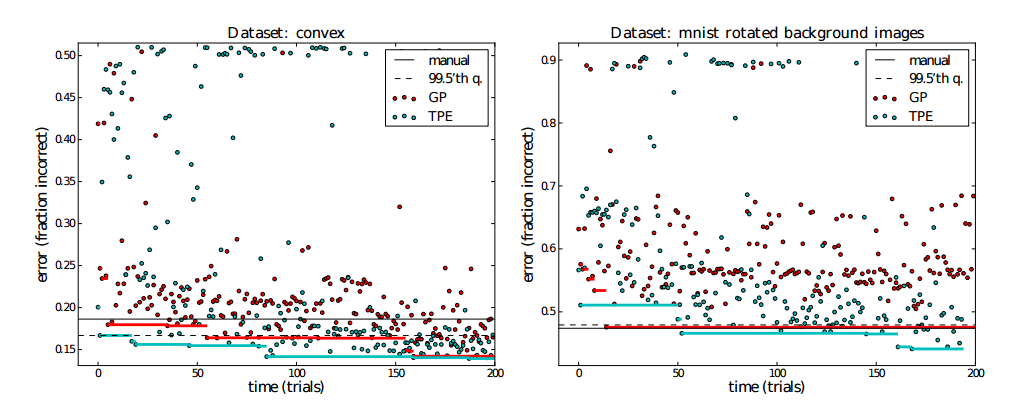
\includegraphics[width =\linewidth]{TPE.png}
    \caption{This image taken from \cite{bergstra2012random} describes in detail the Efficiency of Gaussian Process-based(GP) and graphical model-based(TPE) sequential optimization algorithms on the task of optimizing the validation set performance on two different databases. In the experiment, Both GP and TPE algorithms substantially outperform the manual and random search methods. The performance of TPE is generally higher than GP}
    \label{fig:fig1}
\end{figure}



Figure 1 describes the experimental results described in \cite{bergstra2012random} of the two sequential hyperparameter optimization algorithms on tasks involving DBNs(Deep Belief Networks). There are quite a few possible reasons as to why TPE approach outperformed the GP approach in the two datasets viz. convex and MNIST. All layers were of equal size and the parametric space was of size 32. In this 32-dimensional search problem, the TPE algorithm gave new best results on both the datasets. There are several possible reasons as to why TPE outperformed GP. One possible reason is that that the factorization of $p(x|y)$ is more accurate than $p(y|x)$, or that possibly the exploration induced by TPE's lack of accuracy turned out to be a good heuristic for search. Either way, the important result is that the two sequential algorithms outperformed the random search and human-guided search which have currently are the state of the art.\cite{bergstra2012random}

\end{itemize}

\section{Conclusion}

The paper started with defining Hyper-parameters and discussing how they are essential for tackling problems of \textit{Overfitting}. Next, some common training method and model hyperparameters were listed out and discussed. When appropriate, recommendations for hyperparameter choices were given, which should be taken with a grain of salt. Then the most common heuristics to search and optimize the hyperparameter space were discussed. The Bayesian optimization and Tree-parzen estimator algorithms were the highlight of this paper, since they show great improvement over the classic hyperparameter optimization. They allow learning from the training history and give better estimations for the next set of parameters. Finally, if the optimization of hyper-parameters does not suffice the accuracy needs, more data should be used and ensemble methods should be explored.

\printbibliography
\end{document}